

\documentclass[compress]{beamer}

\usepackage{thumbpdf}
\usepackage{wasysym}
\usepackage{ucs}
\usepackage[utf8]{inputenc}
\usepackage{pgf,pgfarrows,pgfnodes,pgfautomata,pgfheaps,pgfshade}
\usepackage{pgfpages}
\usepackage{verbatim}
\usepackage{fancyvrb}
\usepackage{multimedia}
\usepackage{subcaption}
\usepackage{ulem}
\usepackage{textcomp}
\usepackage{tikz}

\usepackage{listings}

\usepackage{epigraph}
\setlength{\epigraphwidth}{.8\textwidth}

\usepackage{DejaVuSansMono}

\usepackage{multicol}  
\usepackage{media9}

% Adjust the colours to fit your design
\definecolor{mainthemecolour}{rgb}{0.42,0.48,0.37}
\definecolor{mainthemecolourlight}{rgb}{0.63,0.72,0.57}
\definecolor{mainthemecolourstrong}{rgb}{0.40,0.68,0.18}
\definecolor{mid-gray}{gray}{0.7}

\definecolor{greenstrong}{rgb}{0.58,0.77,0.29}
\definecolor{redstrong}{rgb}{0.81,0.22,0.23}
\definecolor{fglisting}{gray}{0.3}
\definecolor{bglisting}{gray}{1}
\definecolor{fgshell}{gray}{1}
\definecolor{bgshell}{gray}{0.1}
\definecolor{bgshelllight}{gray}{0.8}


% Some in-code macros - a bit buggy, but useful
\newcommand{\hl}[1]{\textcolor{greenstrong}{\texttt{#1}}}
\newcommand{\hlErr}[1]{\textcolor{redstrong}{\texttt{#1}}}
\newcommand{\hlOk}[1]{\textcolor{green}{\texttt{#1}}}
\newcommand{\hlInv}[1]{\colorbox{bgshell}{\textcolor{fgshell}{\texttt{#1}}}}

\newcommand{\unhl}[1]{\textcolor{gray}{#1}}
\newcommand{\clda}[0]{$\textcolor{blue}{\lambda}$}
\newcommand{\carr}[0]{$\textcolor{purple}{\rightarrow}$}
\newcommand{\cbind}[0]{\textbf{\texttt{$>\!\!>\!\!=$}}}
\newcommand{\codedots}[0]{\textcolor{mid-gray}{...}}

\usetheme{elegance}

\lstnewenvironment{cxxcode}
    {\lstset
        { escapeinside={@}{@}
        , gobble=8
        , showstringspaces=false
        , basicstyle=\color{fglisting}
        , rulecolor=\color{mainthemecolourlight}
        }
    }
    {}

\lstnewenvironment{cxxcodebox}
    {\lstset
        { escapeinside={@}{@}
        , gobble=6
        , showstringspaces=false
        , basicstyle=\color{fglisting}
        , frame=lr
        , rulecolor=\color{mainthemecolourlight}
        }
    }
    {}

\lstnewenvironment{shellcode}
    {\lstset
        { escapeinside={@}{@}
        , gobble=7
        , showstringspaces=false
        , basicstyle=\color{fgshell}
        , backgroundcolor=\color{bgshell}
        }
    }
    {}


% Marking points to use in Tikz
\usetikzlibrary{arrows,shapes}
\newcommand{\tikzmark}[1]{\tikz[remember picture] \node[coordinate] (#1) {#1};}

% Fragile frames
\newenvironment{xframe}[1][]
  {\begin{frame}[fragile,environment=xframe,#1]}
  {\end{frame}}



\title{\hei{时间序列数据驱动下的深度学习模型研究}}
\subtitle{个人简介与研究课题论证}
\author{张心泽}

\institute{\color{white}
    xinze@hust.edu.cn \\
    https://github.com/XinzeZhang
} %
\date{\footnotesize\color{mainthemecolour} HUST, Wuhan 2018. }



\begin{document}
\hypersetup{pdfpagemode=FullScreen}
\maketitle
\section{Themes}

\subsection{Background images}

\begin{xframe}{Themes for the Elegance}

    You need a \hl{style/images} directory
    with these files inside:

    \begin{itemize}
        \item background-section.pdf
        \item background-slide.pdf
        \item background-title.pdf
        \item logo.png
    \end{itemize}

\end{xframe}


{
\usebackgroundtemplate{
\includegraphics[width=\paperwidth]{../screenshots/theme-1.png}}
\begin{frame}[plain]
    .
\end{frame}
}


{
\usebackgroundtemplate{
\includegraphics[width=\paperwidth]{../screenshots/theme-2.png}}
\begin{frame}[plain]
    .
\end{frame}
}


{
\usebackgroundtemplate{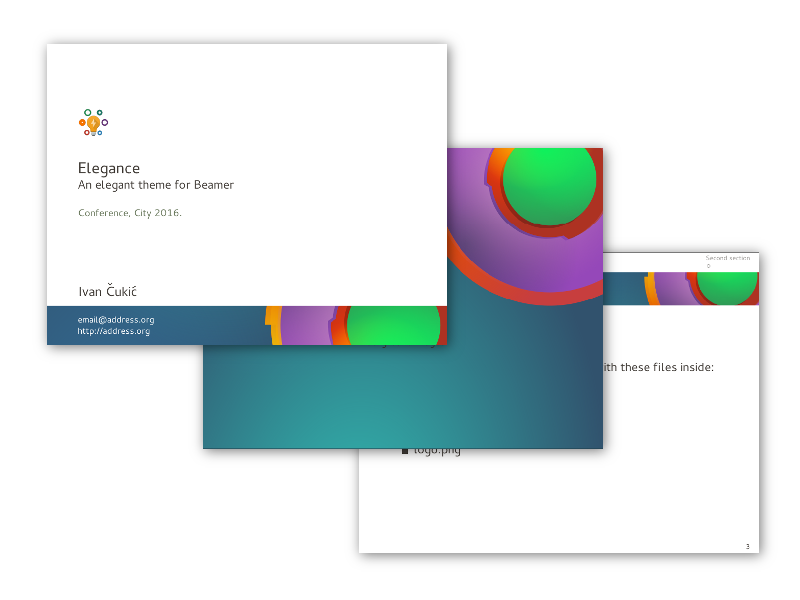
\includegraphics[width=\paperwidth]{../screenshots/theme-3.png}}
\begin{frame}[plain]
    .
\end{frame}
}





\section{Examples}

\subsection{Showing code}

\begin{xframe}{Code snippets}

    Do you have some code to show on the slide?

    And the same frame should also contain text?

    \begin{cxxcodebox}
        class example {
            // \codedots shows grayed-out dots
            @ \codedots @
        };
    \end{cxxcodebox}

    You can use \verb|cxxcodebox| environment.
    It has \verb|cxx| in the name,
    but no syntax highlighting is performed.

    For short code snippets,
    it is better just to highlight the important parts.

\end{xframe}


\subsection{Code slides and escapes}

\begin{xframe}{Second slide}

    \begin{cxxcode}
        class example {
            // There are a few useful escapes here
            @ \codedots @ // \codedots shows grayed-out dots

            // Invalid parts can be marked with \hlErr
            @\hlErr{operator;}@

            // Good parts can be marked with \hlOk
            @\hlOk{operator() ()}@

            // Other highlighting commands can be seen in
            // the preamble.tex file
        };
    \end{cxxcode}

\end{xframe}

\end{document}
